%================================================================================
%       Safety Critical Systems Club - Data Safety Initiative Working Group
%================================================================================
%                       DDDD    SSSS  IIIII  W   W   GGGG
%                       D   D  S        I    W   W  G   
%                       D   D   SSS     I    W W W  G  GG
%                       D   D      S    I    WW WW  G   G
%                       DDDD   SSSS   IIIII  W   W   GGG
%================================================================================
%               Data Safety Guidance Document - LaTeX Source File
%================================================================================
%
% Description:
%   Miscellanea section.
%
%================================================================================
\section{Lifecycle\index{Lifecycle|textbf} Considerations (Discursive)} \label{bkm:lifecycle}

\dsiwgSectionQuote{Failure is an amazing data point that tells you which direction not to go.}{Payal Kadakia}

\subsection{Usage Scenarios}
If safety-related data is incorrect it can become dangerous when used, either by making a computer or control system perform incorrect actions, or by misleading human users into making incorrect decisions. Since the danger can only be determined when the usage of the data is understood, risk assessment should involve both the consumer of the data and the producer.

\begin{figure}[htbp]
  \centering
  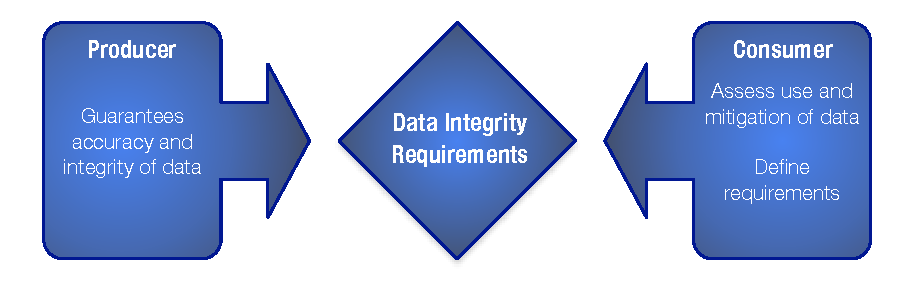
\includegraphics[width=0.75\textwidth]{images/producerconsumer}
  %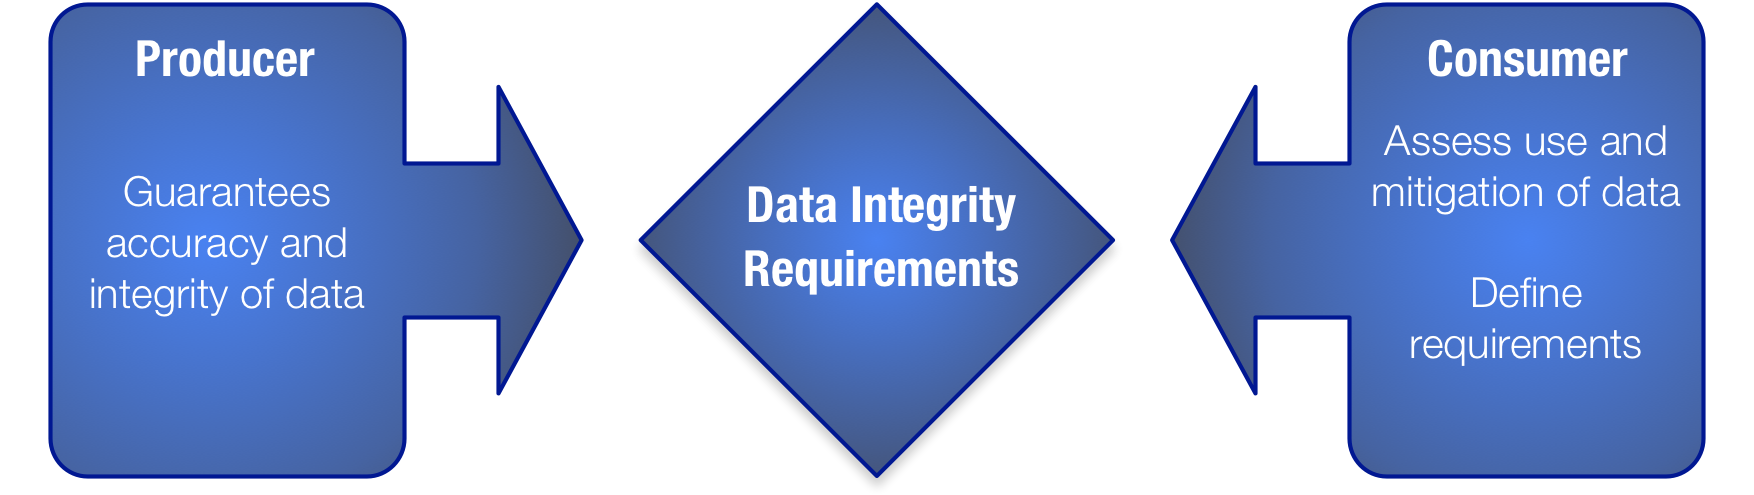
\includegraphics[width=0.75\textwidth]{images/producerconsumer.png}
  \caption{Consumer-focused \index{Integrity Property}integrity requirements}
  \label{fig:producerconsumer}
\end{figure}

The consumer assesses the use of the safety-related data. (In later phases of the Data Safety Management Process this information is used to define the required Data Properties: for example, how accurate a particular safety-related \index{Artefact, Data}Data Artefact must be.)

The producer investigates how the safety-related data is collected and what errors might occur. (Building on activities in later phases of the Data Safety Management Process, the producer can provide some form of guarantee, or level of confidence, that the safety-related data meets the specific data-related requirements.)

In some cases a producer will be providing safety-related data without any knowledge of a specific user (e.g., mapping data or generic databases that are sold to many users). In these cases the producer will need to make some assumptions about possible users, and then clearly state what level of \index{Integrity Property}integrity the data has been produced to. It is then up to the users to check whether the declared \index{Integrity Property}integrity matches their need.

\subsection{Data in System Lifecycles}
Like other components of a safety-related system, the safety dependency of data is dictated by the context in which it is used and the causal links that become established where loss of one or more of the required \index{Property!Data}properties can contribute to hazardous system states. For example, a given data set (say configuration data) could be used in a number of separate contexts such as:
\begin{itemize}
  \item prototyping a system to demonstrate solution feasibility of a safety-related system;
  \item development testing of a safety-related system; and
  \item live operational use of a safety-related system.
\end{itemize}

In these cases, the data set is the same but the context of its use changes the safety significance and therefore the level of assurance that it may require. It follows that the assessed \index{Assurance Level!Data}assurance level of a data set is also predicated on where and when in the lifecycle the data set will be applied. 

To illustrate this concept, a number of generic model lifecycles are discussed below. Note that these are not intended to be prescriptive or mandate the use of any particular model. Instead, they are being used to illustrate how the Data Safety Management Plan could articulate these lifecycle considerations.

\dsiwgTextBF{Development} The diagram in \autoref{fig:developmentlifecycle} represents a typical development lifecycle using an iterative development approach\footnote{The diagram is based on \gls{ibm}'s Rational Unified Process, an iterative software development\index{Software Development Process} process framework. The original diagram is in the public domain.}. In this model there are key phases as the system transitions from concept through to testable executable code. The process is iterative in that several cycles of functional elaboration, design, development and test may be run and these typically will focus on the areas of the system that bear most technical risk or comprise the key functional use cases so the client gets early visibility of the system. This early awareness allows feedback to be provided into the next iteration to help steer the solution to the client's actual needs. Traditional waterfall implementation can map onto this model on the basis that there is only one iteration in each phase and all activities in one phase need to be completed before progressing to the next.

\begin{figure}[htbp]
  \centering
  %\includegraphics[width=\textwidth]{images/developmentlifecycle}
  %\includegraphics[width=\textwidth]{images/developmentlifecycle_png600}
  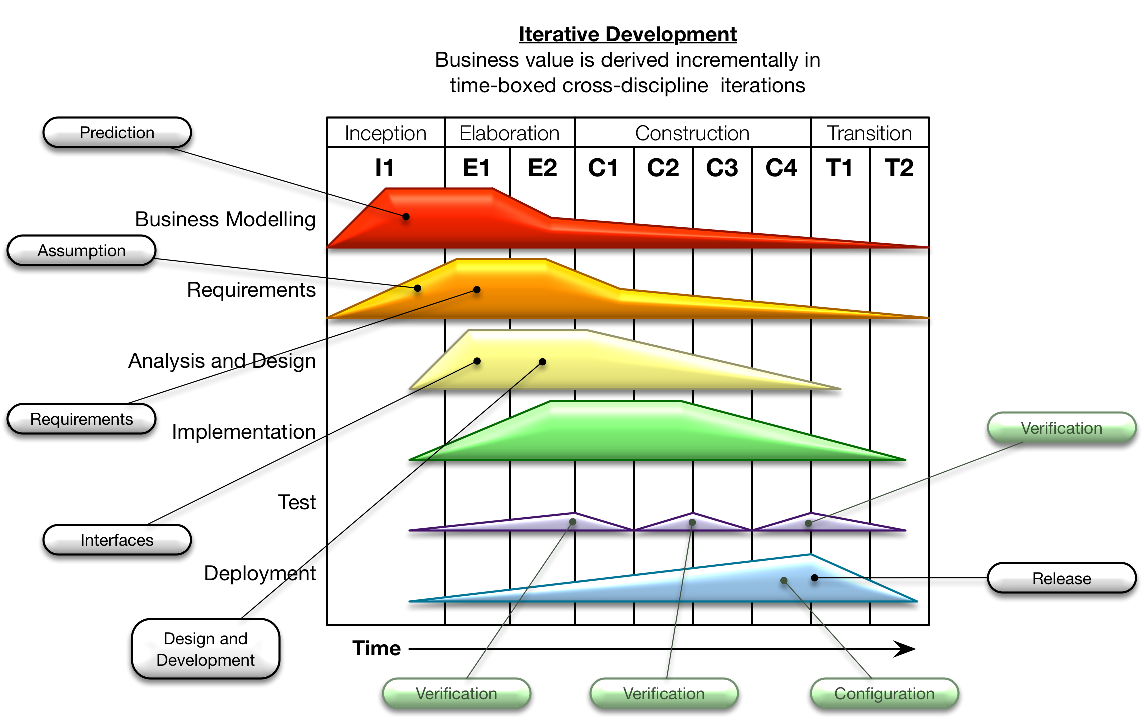
\includegraphics[width=\textwidth]{images/developmentlifecycleflat}
  \caption{Development lifecycle}
  \label{fig:developmentlifecycle}
\end{figure}

The model itself may vary depending on the specific needs of the project but the diagram illustrates that different Data Categories\index{Category!Data} become significant at different points of the process. 

\dsiwgTextBF{Operational} Once a system has been developed it will move into an operational lifecycle or indeed, if data safety has not previously been considered for an enterprise, then the system could already be in operational use. These operational lifecycles tend to be cyclical in nature; the diagram in \autoref{fig:operationallifecycle}\footnote{ITIL is a registered Trade Mark of AXELOS Limited. All rights reserved.} illustrates a typical model.

\begin{figure}[htbp]
  \centering
  %\includegraphics[width=0.9\textwidth]{images/operationallifecycle}
  %\includegraphics[width=0.9\textwidth]{images/operationallifecycle_png600}
  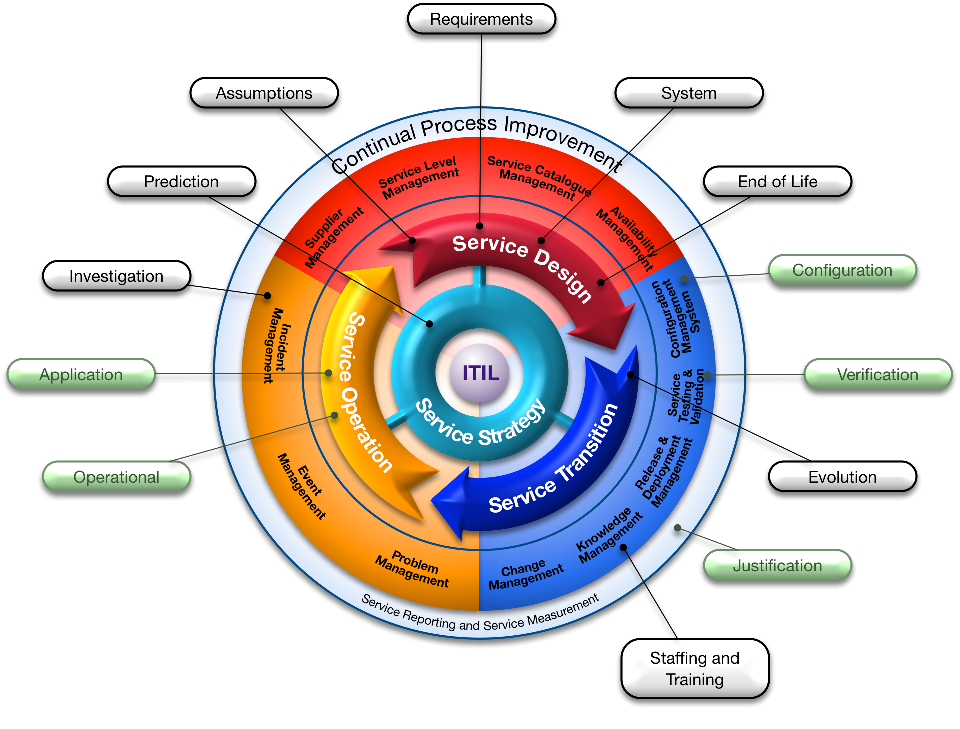
\includegraphics[width=0.9\textwidth]{images/operationallifecycleflat}
  \caption{Operational lifecycle}
  \label{fig:operationallifecycle}
\end{figure}

Again, specific Data \index{Category!Data} will come into play at different periods in the process. Documenting the relationship between process steps and Data Categories will therefore give clarity as to when a particular assurance technique needs to be applied.

\dsiwgTextBF{Data supply chains} The previous models relate to typical system supply and operate perspectives but there are also other data supply chains where a number of organizations engage in the procurement and use of safety-related data. These processes may include the development and operational lifecycles but a different model is required to fully represent the wider processes that are being employed. The diagram in \autoref{fig:dataacquisitionlifecycle} shows such a model representing a data acquisition lifecycle.

\begin{figure}[htbp]
  \centering
  %\includegraphics[width=\textwidth]{images/dataacquisitionlifecycle}
  %\includegraphics[width=\textwidth]{images/dataacquisitionlifecycle_png600}
  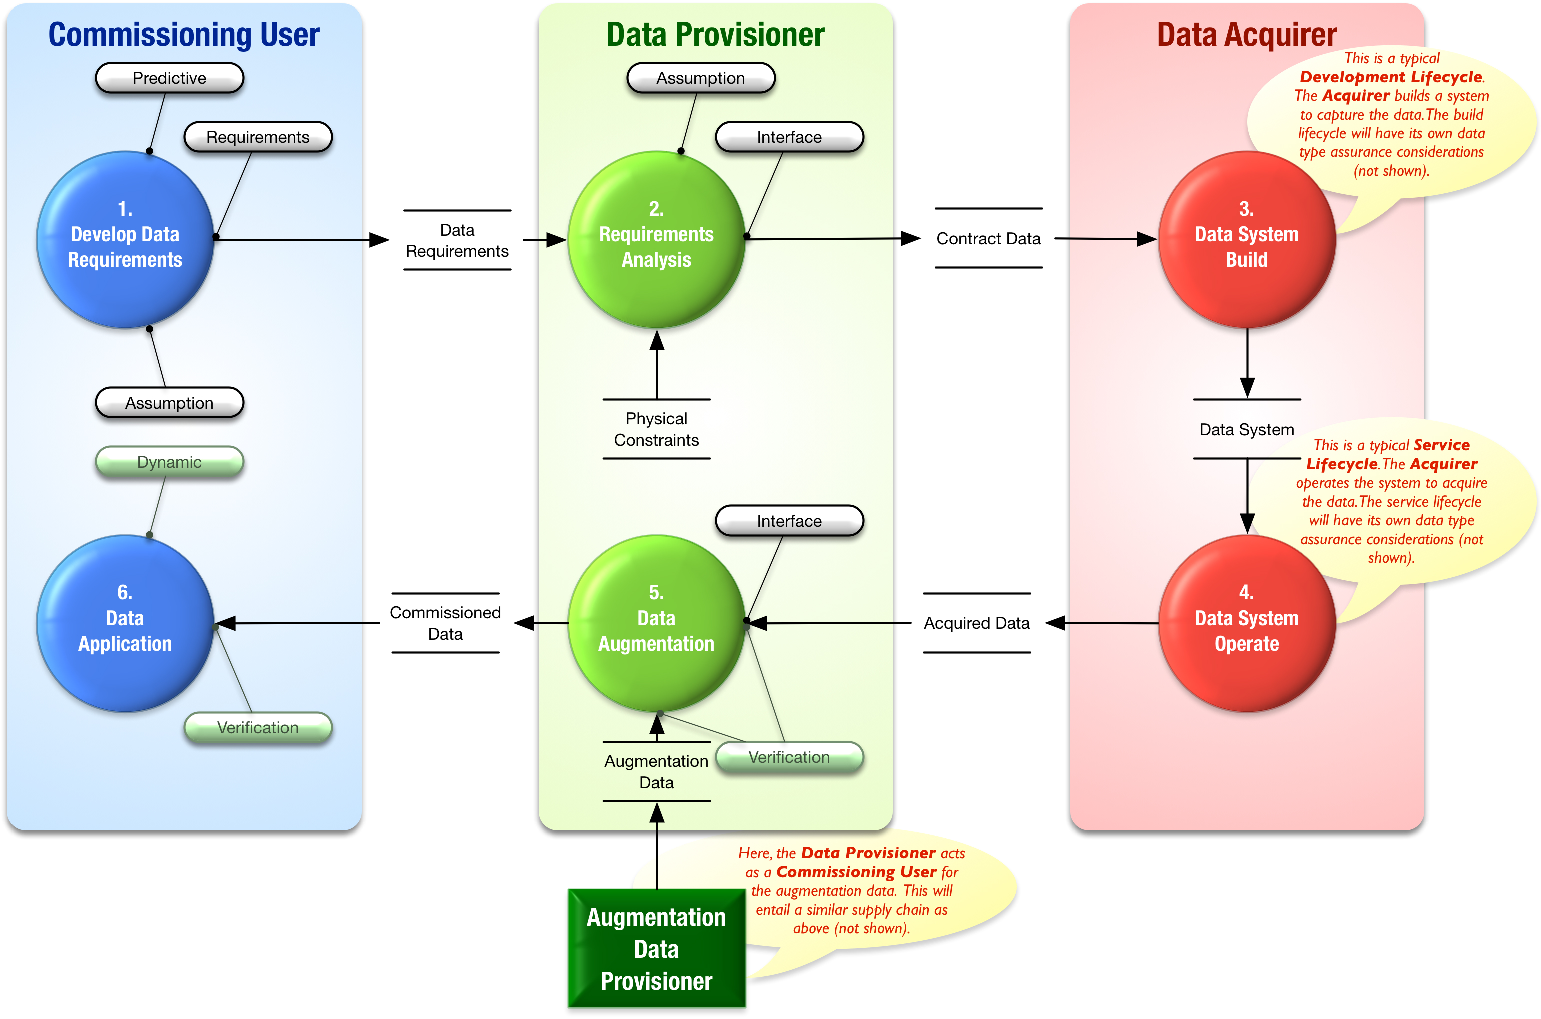
\includegraphics[width=\textwidth]{images/dataacquisitionlifecycleflat}
  \caption{Data supply chain}
  \label{fig:dataacquisitionlifecycle}
\end{figure}

This model represents the interactions between three key organizations:
\begin{itemize}
  \item The Commissioning User: the organization that has the need for the data;
  \item The Data Provisioner: the organization that will fulfil that need for data; and
  \item The Data Acquirer: the organization employed by the Data Provisioner to carry out physical collection of data.
\end{itemize}

Note that these may be three separate organizations, or they may be separate business units within the same, larger, organization.

In this supply chain, the Commissioning User is a Consumer of the data and the Data Acquirer is a Producer of data. The Data Provisioner acts both as a Consumer (from the Data Acquirer) and Producer (to the Commissioning User) of data. Similarly, an organization that augments data sets is both a Consumer and Producer of data in the supply chain.

The Commissioning User Requirement Analysis is the key process step where the Commissioning User's expectations for data (including \index{Fidelity/Representation Property}fidelity levels for associated \index{Property!Data}properties) are agreed with the Data Provisioner. The requirements may be adjusted because of physical constraints (e.g., loss of precision because of physical measuring device constraints) and may include additional requirements to augment the captured data with additional information (e.g., airport codes added to a measurement of a given runway length).

The Data Provisioner may employ a Data Acquirer to capture the data (e.g., to carry out a physical survey of a site). The acquisition phase may itself require a specialised system to be built to perform the capture and data refinement to meet the Data Provisioner's specifications. Such systems will then themselves be subject to the Development lifecycle model considerations discussed above. Likewise, the data augmentation phase may require further system development processes or indeed, could trigger an instance of the model again as the Data Provisioner acting as a Commissioning User.

Acquired and augmented data is then fed into the operational system that has been built for providing the service of generating the commissioned data. This system in its service provision role would then typically follow the Operational Lifecycle process model discussed earlier.

\subsubsection{Tool Assurance}
Tools in this context are considered anything that automates all or part of a process, for example, data creation or data transformation. Test tools are also included (i.e., the term is not limited to parts of an operational system).

Tools can impact data safety in different ways, depending on both their function and how they are to be used. For tools to be considered fit for purpose it is necessary to show that the tool meets its requirements in the context in which it is to be used. The activity to ensure a tool is fit for purpose is usually called ``tool qualification''.

The first step is to define the purpose for which the tool is required to be fit. Once that is done, and the tool's requirements are specified, there are three main strategies available for qualification:
\begin{itemize}
  \item Use evidence of a previous certification of the tool by a trusted third party (unlikely to be available in most industry sectors);
  \item Base tool qualification on the practices used when designing and developing the tool (only practicable for tools developed within the organization); and
  \item Use one of the available industry-specific guidance documents that admit \gls{cots} solutions, e.g., EUROCAE Document ED-215 (RTCA/DO-330) \cite{citation:ED215}.
\end{itemize}

%There is an alternative, risk-based and perhaps more feasible, approach. This involves assessing the potential risks presented by use of the tool and providing assurance that these risks are adequately managed. The method proceeds as follows:

%\begin{itemize}
%  \item Draft a procedure for the use of the tool to achieve the stated purpose;
%  \item Identify threats to data safety associated with using the tool;
%  \item Specify adequate mitigations\index{Mitigation} for each identified threat;
%  \item Augment and formally issue the tool requirements and the usage procedure to implement the specified  mitigations\index{Mitigation%};
%  \item Demonstrate that the tool and its mitigations\index{Mitigation} perform as expected; and
%  \item Provide a compelling assurance argument based on the previous steps and any other evidence that will improve confidence; for example:
%  \begin{itemize}
%    \item reputation of the supplier; 
%    \item configuration management of the tool, its settings and its documentation;
%    \item competence of the tool user; and
%    \item checks that are made on the tool's output.
%   \end{itemize}
%\end{itemize}

Further details on tool qualification are presented in \dsiwgRef{Appendix}{bkm:tools}.

\subsubsection{Test Data}
The generation of suitable test data is critical to verification of a safety system. The test data must include both representative ``normal'' values based on intended usage and also values which push at, and beyond, normal use to provoke hazards that the system might produce. This latter type of test data is particularly hard to generate: generally it must be credible, yet it must stress the system to react in a way that the preservation of \index{Property!Safety}safety properties can be assessed. 

In general, all the \index{Property!Data}properties of the test data should be considered and an assessment made as to whether breaking a property (e.g., introducing corrupt or late data) would cause a problem to the system. If it does, then specific test data should be produced to facilitate testing of this potential problem.

Some suggestions for test data for safety-related systems are:
\begin{itemize}
  \item Use of values on or around boundaries;
  \item Use of extreme values, way beyond what could be reasonably expected;
  \item Use of typical ``everyday'' values / sets;
  \item Some realistic but unexpected values;
  \item Try combinations of data values or items that are problematic together (e.g., inconsistent);
  \item If possible, use some values known to have caused problems in the past;
  \item Where appropriate, use values related to timing, rollover or date boundaries;
  \item Where possible, use white box values (i.e., those derived from an understanding of the system);
  \item Use a set of values with drift or bias over time;
  \item Use data sets with particular \index{Property!Statistical}statistical properties (e.g., distribution, patterns etc.);
  \item Use data which has incorrect formatting, ordering, or out of sequence, etc.; and
  \item Try data which has repeated sets of values or pseudo-random characteristics.
\end{itemize}
Typically very complex test data is derived from recorded live feeds of real data flows. While this data can be extremely useful for regression purposes, it should be recognised that it is unlikely to contain many outlying or boundary data items. Therefore it may need to be modified to test any hazardous situations; this modification can be difficult and may require sophisticated tools to both ensure correct \index{Property!Data}properties and injection of the intended faults (for instance to introduce a statistical bias to the data).

Simulator / emulator derived values can be useful, but again the issue is how realistic the values are: often the \index{Accuracy Property}\gls{accuracy}, resolution or timing of simulated values may be different to real data.

Coverage with test data is something to consider. Sometimes the same data set is used for multiple test scenarios, when in fact it is not stressing all of them to the same degree. Test data coverage can be collected over requirements, code or design, but it is important not to forget hazards: coverage of the hazards and mitigations\index{Mitigation} identified in the hazard log is a key aim. 

In general some measure of the quality and suitability of the test data can be useful. This could be based on {Property!Statistical}statistical properties, coverage of hazards or coverage of requirements. 

Test data must show continued relevance, through systems evolution\index{Evolution!System} and over time. It is good practice to build up extensive regression suites containing coverage of all detected problems to date.

\subsubsection{Interfaces with Existing Assessments}\index{Interface!Assessment}
\paragraph{Data and Software}\index{Software vs. Data}
Although most people feel they have an intuitive understanding of the difference between software and data, upon closer examination the boundary is not always as clear as it may first appear.

Consider, for example, Java bytecode, which is operated on by a Java Virtual Machine. From one perspective, it could be argued that the Java bytecode is simply data. By extension, it could also be argued that the Java source code is also just data. This type of argument can be extended to suggest that any software\index{Software vs. Data} can, at least from one viewpoint, be considered as data. Conversely, think about the data used in a 3D printer, perhaps to produce a part for an aircraft. This data could be viewed as a program for the printer; that is, it could potentially be viewed as software. This type of argument can easily be extended across a range of situations, especially those relating to configuration data.

While they are interesting, and potentially important, these philosophical considerations should not detract from the practical issue: there are some aspects of data (using the term in a generic sense) that are often not explicitly addressed in standards. These are a consequence of features that are more readily apparent in data than in software\index{Software vs. Data}. Examples include:
\begin{itemize}
  \item It is easy for data to be reused in a range of contexts and despite appearances it is not trivial to translate an assurance argument that the data is fit for purpose from one context to another.
  \item It is not always clear who owns or is responsible for data, especially when data is shared and processed amongst a collection of disparate systems.
	\item Data often has a lifetime, that is a time after which it is no longer valid. This may be a strict cut off, or a more gradual degradation in the utility (or applicability) of the data.
  \item There is often a default value for data. While this can make systems easier to use and hence more productive it can be difficult to identify a default value that is appropriate for all circumstances.
  \item It can be easy to change data. In some circumstances this can give rise to a temptation to make uncontrolled and potentially untested changes. It can also allow data to be fraudulently changed after an accident.
\end{itemize}
In summary, data and software\index{Software vs. Data} are closely related and, as such, need to be considered together in system engineering activities, including system safety analyses. However, data and software emphasise different facets of risk and they are susceptible to different mitigation\index{Mitigation} approaches; this means there is also a need to adopt a data-focused perspective. It also means that \cbstart\index{Assurance Level!Software}\glspl{software assurance level}\cbend\ cannot be mapped directly to \index{Assurance Level!Data}\glspl{dsal}.

\paragraph{Data Safety and Security}
When generating high-level processes and techniques to manage the risks posed by data, it is worthwhile understanding the difference between the safety risks posed by accidental failure to preserve \index{Property!Data}Data Properties and the security risks posed by actors maliciously undermining the properties of data.

The relationship between safety and security, as engineering concepts, can be summarised by their relationships to cultural, developmental and aspirational \index{Property!System Development}properties of systems development.

Culturally, embedding both safety and security into an organization is seen as a key strategic goal for creating systems that are both safe and secure. Developmentally, safety and security are quality factors, generating transverse requirements that impact the entire system. Most importantly, at the aspirational level, both safety and security have the common goal of preventing harm from accidental and malicious interventions respectively.

For an organization aiming to create systems that are both safe and secure, these connections can be both a benefit and a burden. The shared goal of preventing harm means that both quality factors seek to identify routes to harm through analysis of the system being developed. This can result in shared processes and tools, which in turn can save time and money during systems development. However, safety and security interact in a more volatile way at the functional level. Security failings can undermine the safety case for a system and, conversely, \index{Safety Requirement}safety requirements can prevent the implementation of standard security solutions. For example, the German government published a report in 2014 into a fire at a steel works caused by a cyber attack that resulted in the control system being placed into an unsafe state and the safety system being unable to intervene (Section 3.3.1 of \cite{citation:DieLage} - in German). In addition, ``fail-safe'' states can often leave a system with exposed security vulnerabilities.

These links between safety and security infer that there are connections between the sub-categories of data safety and information security: both attempt to take a data-centric view of the system of interest in order to improve the associated quality factor; and both attempt to prevent harm through the preservation of the \index{Property!Data}properties of data within that system.

In the security domain, the three key properties of data considered are confidentiality, \index{Integrity Property}integrity, and \gls{availability}. Confidentiality, the failure of which is termed ``Information Disclosure'' in the Microsoft Security Model, \cite{citation:leblanc2002writing} is typically not a safety concern as, without malicious intent, information sharing is not inherently unsafe. However, when considering systems where confidentiality is an important property, the interaction between data safety and security cannot be trivially resolved. For example, accidental disclosure of information can form part of a causal chain which leads to harm from a malicious actor.

Data \index{Integrity Property}integrity is a critical property for both domains. The Microsoft Security Model describes malicious removal of the property of \index{Integrity Property}integrity as ``tampering''. Whether by accident or through malicious intent, the potential harm from loss of data \index{Integrity Property}integrity can be disastrous to a safety-critical system, from the values of drug dosages to control system parameters. 

Data \gls{availability} is also important to both domains. Loss of \gls{availability}, or ``denial of service'' in the Microsoft Security Model, is another \index{Property!Data}property that can be lost accidentally or through malicious intervention. Loss of \gls{availability} prevents systems from functioning properly and can result in undefined behaviour if not mitigated\index{Mitigation} by design.

Further guidance on the integration of safety and security can be found in a Code of Practice published by the IET
\cite{citation:IetCyber}.
The Code of Practice is written for engineers and engineering management to support their understanding of the issues
involved in ensuring that the safety responsibilities of an organization are addressed, in the presence of a threat of
cyber attack.
